% Created by tikzDevice version 0.10.1 on 2017-09-04 20:14:48
% !TEX encoding = UTF-8 Unicode
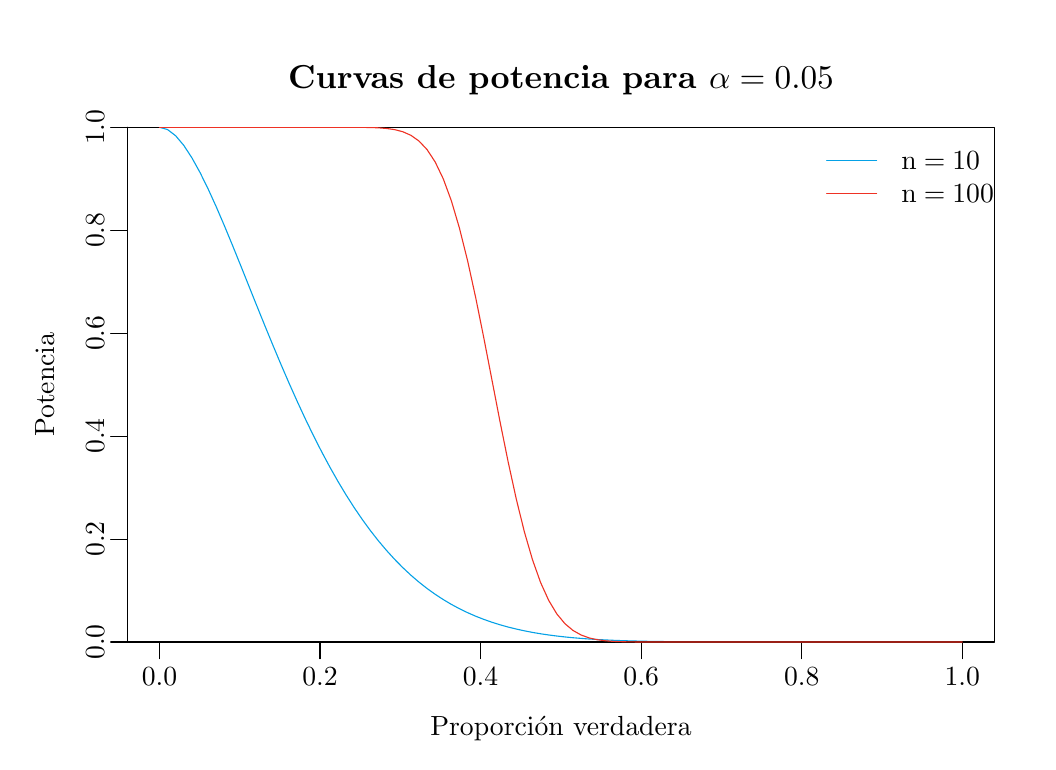
\begin{tikzpicture}[x=1pt,y=1pt]
\definecolor{fillColor}{RGB}{255,255,255}
\path[use as bounding box,fill=fillColor,fill opacity=0.00] (0,0) rectangle (361.35,258.00);
\begin{scope}
\path[clip] ( 36.00, 36.00) rectangle (349.35,222.00);
\definecolor{drawColor}{RGB}{5,161,230}

\path[draw=drawColor,line width= 0.4pt,line join=round,line cap=round] ( 47.61,222.00) --
	( 50.54,221.19) --
	( 53.47,218.94) --
	( 56.40,215.47) --
	( 59.33,210.99) --
	( 62.26,205.70) --
	( 65.19,199.76) --
	( 68.12,193.32) --
	( 71.05,186.50) --
	( 73.98,179.43) --
	( 76.91,172.19) --
	( 79.84,164.88) --
	( 82.77,157.57) --
	( 85.70,150.32) --
	( 88.64,143.18) --
	( 91.57,136.21) --
	( 94.50,129.43) --
	( 97.43,122.88) --
	(100.36,116.57) --
	(103.29,110.53) --
	(106.22,104.77) --
	(109.15, 99.30) --
	(112.08, 94.12) --
	(115.01, 89.24) --
	(117.94, 84.64) --
	(120.87, 80.34) --
	(123.80, 76.32) --
	(126.73, 72.58) --
	(129.67, 69.10) --
	(132.60, 65.88) --
	(135.53, 62.91) --
	(138.46, 60.17) --
	(141.39, 57.65) --
	(144.32, 55.35) --
	(147.25, 53.25) --
	(150.18, 51.34) --
	(153.11, 49.60) --
	(156.04, 48.03) --
	(158.97, 46.61) --
	(161.90, 45.33) --
	(164.83, 44.18) --
	(167.76, 43.15) --
	(170.69, 42.23) --
	(173.63, 41.41) --
	(176.56, 40.69) --
	(179.49, 40.05) --
	(182.42, 39.48) --
	(185.35, 38.98) --
	(188.28, 38.55) --
	(191.21, 38.17) --
	(194.14, 37.84) --
	(197.07, 37.55) --
	(200.00, 37.31) --
	(202.93, 37.09) --
	(205.86, 36.91) --
	(208.79, 36.76) --
	(211.72, 36.62) --
	(214.66, 36.51) --
	(217.59, 36.42) --
	(220.52, 36.34) --
	(223.45, 36.27) --
	(226.38, 36.22) --
	(229.31, 36.18) --
	(232.24, 36.14) --
	(235.17, 36.11) --
	(238.10, 36.09) --
	(241.03, 36.07) --
	(243.96, 36.05) --
	(246.89, 36.04) --
	(249.82, 36.03) --
	(252.75, 36.02) --
	(255.68, 36.02) --
	(258.62, 36.01) --
	(261.55, 36.01) --
	(264.48, 36.01) --
	(267.41, 36.00) --
	(270.34, 36.00) --
	(273.27, 36.00) --
	(276.20, 36.00) --
	(279.13, 36.00) --
	(282.06, 36.00) --
	(284.99, 36.00) --
	(287.92, 36.00) --
	(290.85, 36.00) --
	(293.78, 36.00) --
	(296.71, 36.00) --
	(299.65, 36.00) --
	(302.58, 36.00) --
	(305.51, 36.00) --
	(308.44, 36.00) --
	(311.37, 36.00) --
	(314.30, 36.00) --
	(317.23, 36.00) --
	(320.16, 36.00) --
	(323.09, 36.00) --
	(326.02, 36.00) --
	(328.95, 36.00) --
	(331.88, 36.00) --
	(334.81, 36.00) --
	(337.74, 36.00);
\end{scope}
\begin{scope}
\path[clip] (  0.00,  0.00) rectangle (361.35,258.00);
\definecolor{drawColor}{RGB}{0,0,0}

\path[draw=drawColor,line width= 0.4pt,line join=round,line cap=round] ( 47.61, 36.00) -- (337.74, 36.00);

\path[draw=drawColor,line width= 0.4pt,line join=round,line cap=round] ( 47.61, 36.00) -- ( 47.61, 30.00);

\path[draw=drawColor,line width= 0.4pt,line join=round,line cap=round] (105.63, 36.00) -- (105.63, 30.00);

\path[draw=drawColor,line width= 0.4pt,line join=round,line cap=round] (163.66, 36.00) -- (163.66, 30.00);

\path[draw=drawColor,line width= 0.4pt,line join=round,line cap=round] (221.69, 36.00) -- (221.69, 30.00);

\path[draw=drawColor,line width= 0.4pt,line join=round,line cap=round] (279.72, 36.00) -- (279.72, 30.00);

\path[draw=drawColor,line width= 0.4pt,line join=round,line cap=round] (337.74, 36.00) -- (337.74, 30.00);

\node[text=drawColor,anchor=base,inner sep=0pt, outer sep=0pt, scale=  1.00] at ( 47.61, 20.40) {0.0};

\node[text=drawColor,anchor=base,inner sep=0pt, outer sep=0pt, scale=  1.00] at (105.63, 20.40) {0.2};

\node[text=drawColor,anchor=base,inner sep=0pt, outer sep=0pt, scale=  1.00] at (163.66, 20.40) {0.4};

\node[text=drawColor,anchor=base,inner sep=0pt, outer sep=0pt, scale=  1.00] at (221.69, 20.40) {0.6};

\node[text=drawColor,anchor=base,inner sep=0pt, outer sep=0pt, scale=  1.00] at (279.72, 20.40) {0.8};

\node[text=drawColor,anchor=base,inner sep=0pt, outer sep=0pt, scale=  1.00] at (337.74, 20.40) {1.0};

\path[draw=drawColor,line width= 0.4pt,line join=round,line cap=round] ( 36.00, 36.00) -- ( 36.00,222.00);

\path[draw=drawColor,line width= 0.4pt,line join=round,line cap=round] ( 36.00, 36.00) -- ( 30.00, 36.00);

\path[draw=drawColor,line width= 0.4pt,line join=round,line cap=round] ( 36.00, 73.20) -- ( 30.00, 73.20);

\path[draw=drawColor,line width= 0.4pt,line join=round,line cap=round] ( 36.00,110.40) -- ( 30.00,110.40);

\path[draw=drawColor,line width= 0.4pt,line join=round,line cap=round] ( 36.00,147.60) -- ( 30.00,147.60);

\path[draw=drawColor,line width= 0.4pt,line join=round,line cap=round] ( 36.00,184.80) -- ( 30.00,184.80);

\path[draw=drawColor,line width= 0.4pt,line join=round,line cap=round] ( 36.00,222.00) -- ( 30.00,222.00);

\node[text=drawColor,rotate= 90.00,anchor=base,inner sep=0pt, outer sep=0pt, scale=  1.00] at ( 27.60, 36.00) {0.0};

\node[text=drawColor,rotate= 90.00,anchor=base,inner sep=0pt, outer sep=0pt, scale=  1.00] at ( 27.60, 73.20) {0.2};

\node[text=drawColor,rotate= 90.00,anchor=base,inner sep=0pt, outer sep=0pt, scale=  1.00] at ( 27.60,110.40) {0.4};

\node[text=drawColor,rotate= 90.00,anchor=base,inner sep=0pt, outer sep=0pt, scale=  1.00] at ( 27.60,147.60) {0.6};

\node[text=drawColor,rotate= 90.00,anchor=base,inner sep=0pt, outer sep=0pt, scale=  1.00] at ( 27.60,184.80) {0.8};

\node[text=drawColor,rotate= 90.00,anchor=base,inner sep=0pt, outer sep=0pt, scale=  1.00] at ( 27.60,222.00) {1.0};

\path[draw=drawColor,line width= 0.4pt,line join=round,line cap=round] ( 36.00, 36.00) --
	(349.35, 36.00) --
	(349.35,222.00) --
	( 36.00,222.00) --
	( 36.00, 36.00);
\end{scope}
\begin{scope}
\path[clip] (  0.00,  0.00) rectangle (361.35,258.00);
\definecolor{drawColor}{RGB}{0,0,0}

\node[text=drawColor,anchor=base,inner sep=0pt, outer sep=0pt, scale=  1.20] at (192.68,235.86) {\bfseries Curvas de potencia para $\alpha = 0.05$};

\node[text=drawColor,anchor=base,inner sep=0pt, outer sep=0pt, scale=  1.00] at (192.68,  2.40) {Proporción verdadera};

\node[text=drawColor,rotate= 90.00,anchor=base,inner sep=0pt, outer sep=0pt, scale=  1.00] at (  9.60,129.00) {Potencia};
\end{scope}
\begin{scope}
\path[clip] ( 36.00, 36.00) rectangle (349.35,222.00);
\definecolor{drawColor}{RGB}{238,50,36}

\path[draw=drawColor,line width= 0.4pt,line join=round,line cap=round] ( 47.61,222.00) --
	( 50.54,222.00) --
	( 53.47,222.00) --
	( 56.40,222.00) --
	( 59.33,222.00) --
	( 62.26,222.00) --
	( 65.19,222.00) --
	( 68.12,222.00) --
	( 71.05,222.00) --
	( 73.98,222.00) --
	( 76.91,222.00) --
	( 79.84,222.00) --
	( 82.77,222.00) --
	( 85.70,222.00) --
	( 88.64,222.00) --
	( 91.57,222.00) --
	( 94.50,222.00) --
	( 97.43,222.00) --
	(100.36,222.00) --
	(103.29,222.00) --
	(106.22,222.00) --
	(109.15,222.00) --
	(112.08,222.00) --
	(115.01,222.00) --
	(117.94,221.99) --
	(120.87,221.97) --
	(123.80,221.92) --
	(126.73,221.81) --
	(129.67,221.58) --
	(132.60,221.16) --
	(135.53,220.40) --
	(138.46,219.11) --
	(141.39,217.05) --
	(144.32,213.94) --
	(147.25,209.47) --
	(150.18,203.36) --
	(153.11,195.40) --
	(156.04,185.50) --
	(158.97,173.75) --
	(161.90,160.40) --
	(164.83,145.87) --
	(167.76,130.73) --
	(170.69,115.58) --
	(173.63,101.04) --
	(176.56, 87.65) --
	(179.49, 75.79) --
	(182.42, 65.72) --
	(185.35, 57.49) --
	(188.28, 51.03) --
	(191.21, 46.16) --
	(194.14, 42.63) --
	(197.07, 40.17) --
	(200.00, 38.53) --
	(202.93, 37.48) --
	(205.86, 36.83) --
	(208.79, 36.45) --
	(211.72, 36.23) --
	(214.66, 36.12) --
	(217.59, 36.05) --
	(220.52, 36.02) --
	(223.45, 36.01) --
	(226.38, 36.00) --
	(229.31, 36.00) --
	(232.24, 36.00) --
	(235.17, 36.00) --
	(238.10, 36.00) --
	(241.03, 36.00) --
	(243.96, 36.00) --
	(246.89, 36.00) --
	(249.82, 36.00) --
	(252.75, 36.00) --
	(255.68, 36.00) --
	(258.62, 36.00) --
	(261.55, 36.00) --
	(264.48, 36.00) --
	(267.41, 36.00) --
	(270.34, 36.00) --
	(273.27, 36.00) --
	(276.20, 36.00) --
	(279.13, 36.00) --
	(282.06, 36.00) --
	(284.99, 36.00) --
	(287.92, 36.00) --
	(290.85, 36.00) --
	(293.78, 36.00) --
	(296.71, 36.00) --
	(299.65, 36.00) --
	(302.58, 36.00) --
	(305.51, 36.00) --
	(308.44, 36.00) --
	(311.37, 36.00) --
	(314.30, 36.00) --
	(317.23, 36.00) --
	(320.16, 36.00) --
	(323.09, 36.00) --
	(326.02, 36.00) --
	(328.95, 36.00) --
	(331.88, 36.00) --
	(334.81, 36.00) --
	(337.74, 36.00);
\definecolor{drawColor}{RGB}{5,161,230}

\path[draw=drawColor,line width= 0.4pt,line join=round,line cap=round] (288.72,210.00) -- (306.72,210.00);
\definecolor{drawColor}{RGB}{238,50,36}

\path[draw=drawColor,line width= 0.4pt,line join=round,line cap=round] (288.72,198.00) -- (306.72,198.00);
\definecolor{drawColor}{RGB}{0,0,0}

\node[text=drawColor,anchor=base west,inner sep=0pt, outer sep=0pt, scale=  1.00] at (315.72,206.80) {n};

\node[text=drawColor,anchor=base west,inner sep=0pt, outer sep=0pt, scale=  1.00] at (323.82,206.80) {=};

\node[text=drawColor,anchor=base west,inner sep=0pt, outer sep=0pt, scale=  1.00] at (334.14,206.80) {10};

\node[text=drawColor,anchor=base west,inner sep=0pt, outer sep=0pt, scale=  1.00] at (315.72,194.80) {n};

\node[text=drawColor,anchor=base west,inner sep=0pt, outer sep=0pt, scale=  1.00] at (323.82,194.80) {=};

\node[text=drawColor,anchor=base west,inner sep=0pt, outer sep=0pt, scale=  1.00] at (334.14,194.80) {100};
\end{scope}
\end{tikzpicture}
